\documentclass[a4paper,11pt]{article}
\usepackage{graphicx}
\usepackage{booktabs}
\usepackage{setspace}
\usepackage{parskip}
\usepackage{float}
\onehalfspacing
\begin{document}

\author{Henri Bunting (358718) \and Malte Seimers (378120)}
\title{\vspace{-2cm}Report for Sheet 1\\
\small{Lab Course Machine Learning and Data Analysis}}
\maketitle

\section*{Implementation comments}
The goal of the assignment was to implement and play with two forms of dimensionality reduction: PCA and LLE, an evaluation method for classifiers: AUC / ROC, and a distance measure: the gamma index.

We passed all tests.

Unfortunately, we did not have time to finish Assignment 8.

\section*{Exercise 1 - Implement PCA}
Exercise 1 was pretty straight forward.  We got a bit confused about the orientation of each of the different matrices, but got it sorted out in the end.  Initially, we used np.linalg.eig to compute the eigen vectors / values, but got imaginary results later on so we switched to np.linalg.eigh.  

\section*{Exercise 2 - Implement gamma index}
Gamma index went quickly.  We made our own K-Nearest neighbors algorithm.

\section*{Exercise 3 - Implement AUC}
We came up with two different implementations for AUC.  One is with a for loop, iterating over each point as a bias, and the over was using cumsum and taking a dot product.  The non-loop implementation was of course faster, about 80\% of the speed of the loop version.

\section*{Exercise 4 - Implement LLE}
This was the most difficult of all the implementations.  We got a bit confused what that the tolerance was the regularization parameter.
\clearpage
\section*{Exercise 5 - Application PCA}


\subsection*{No noise}
\begin{figure}[H]
\minipage{0.39\textwidth}
  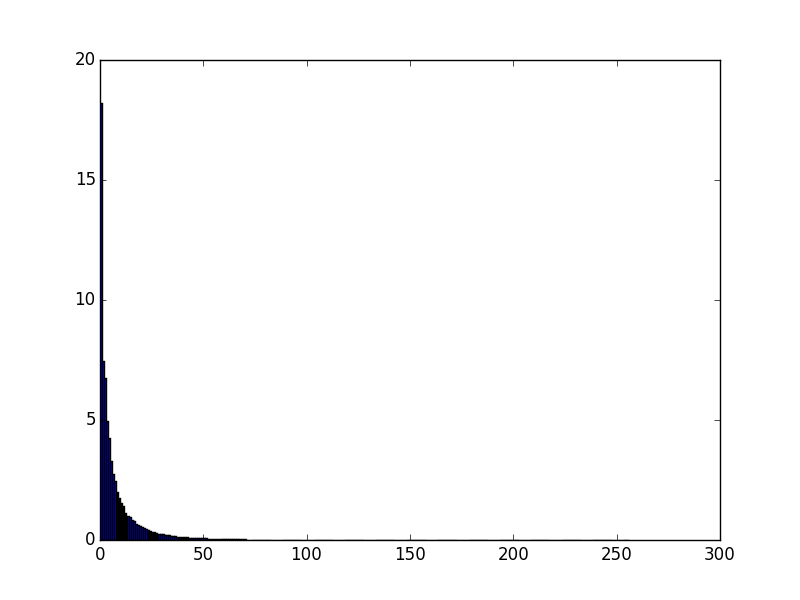
\includegraphics[width=\linewidth]{5_b_a_00.png}
  \caption{All PCs}\label{fig:awesome_image1}
\endminipage\hfill
\minipage{0.39\textwidth}
  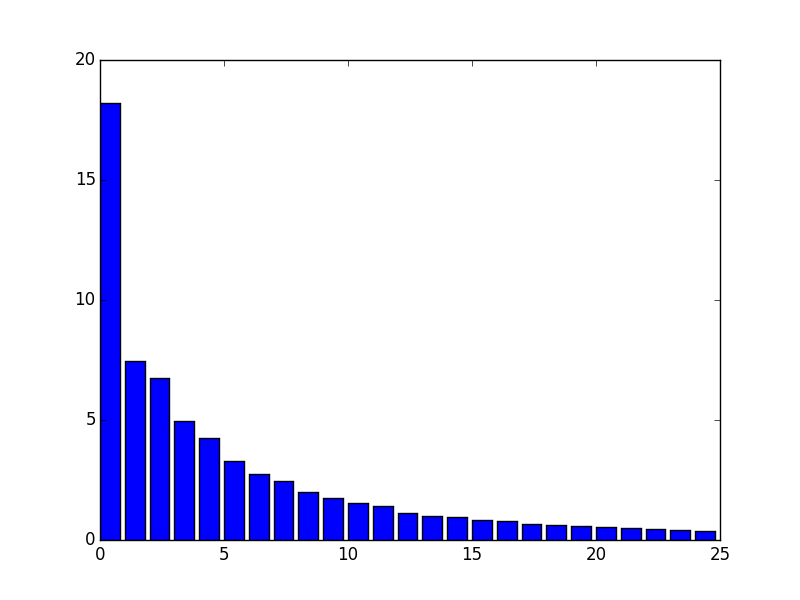
\includegraphics[width=\linewidth]{5_b_b_00.png}
  \caption{First 25 PCs}\label{fig:awesome_image2}
\endminipage\hfill
\minipage{0.20\textwidth}%
  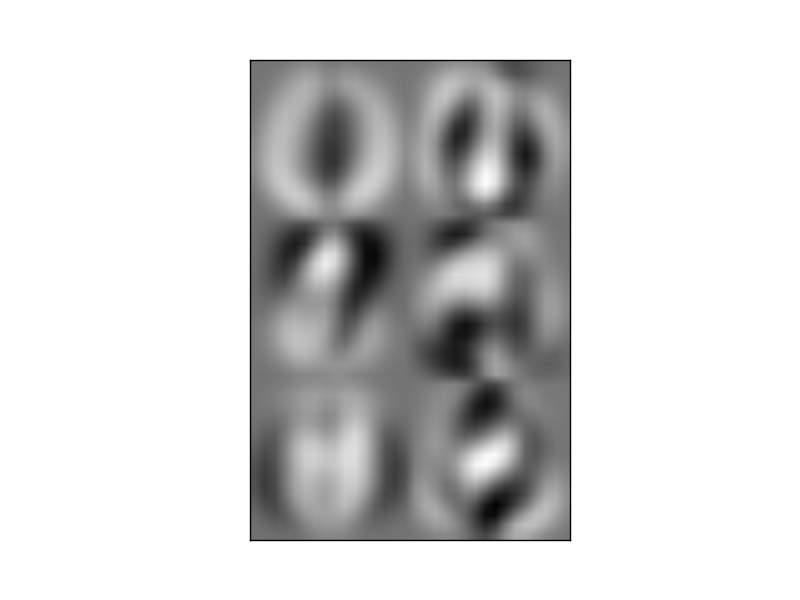
\includegraphics[width=\linewidth]{5_b_c_00.png}
  \caption{First 6 PCs}\label{fig:awesome_image3}
\endminipage
\end{figure}

\begin{figure}[H]
  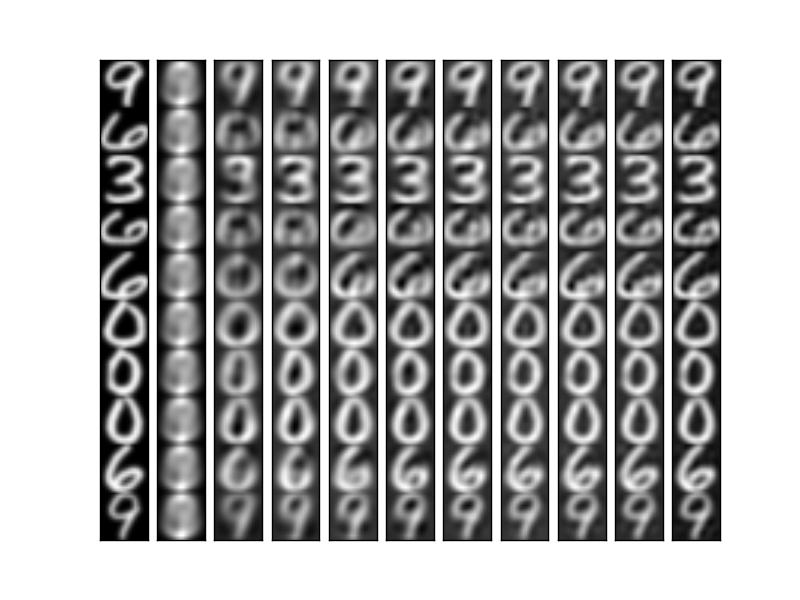
\includegraphics[width=\linewidth]{5_c_Xprime_00_45_allinone.png}
  \caption{Orginal 10 images, followed by 0, 5, 10, ... PCs}\label{fig:6}
\end{figure}


\subsection*{Low noise (X + .5*noise)}
\begin{figure}[H]

\minipage{0.39\textwidth}
  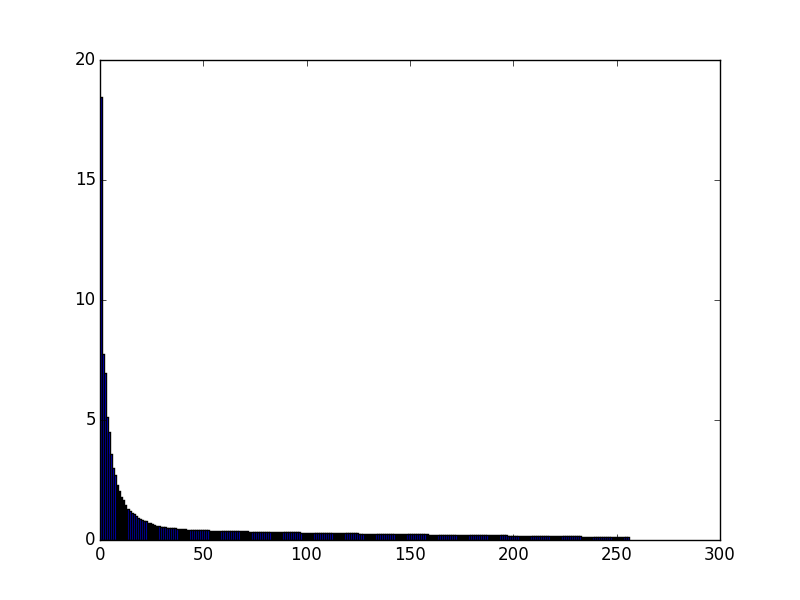
\includegraphics[width=\linewidth]{5_b_a_05.png}
  \caption{All PCs}\label{fig:awesome_image1}
\endminipage\hfill
\minipage{0.39\textwidth}
  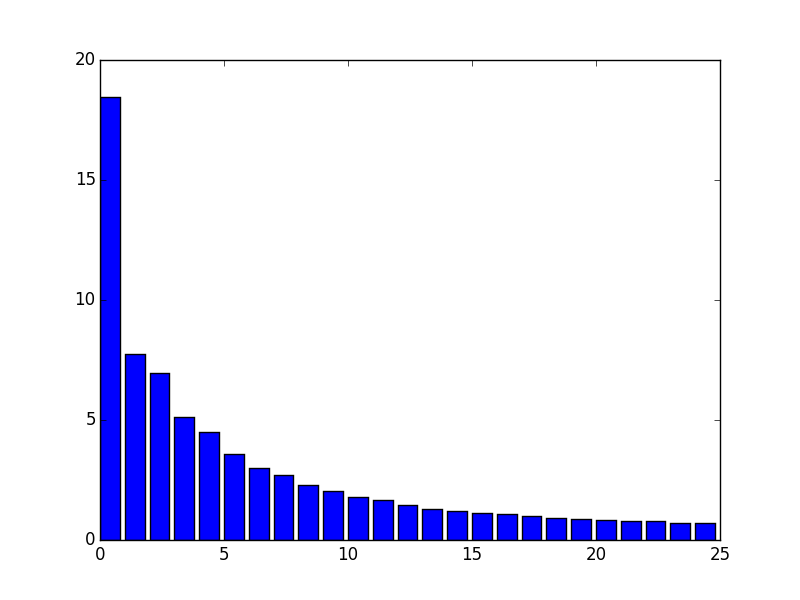
\includegraphics[width=\linewidth]{5_b_b_05.png}
  \caption{First 25 PCs}\label{fig:awesome_image2}
\endminipage\hfill
\minipage{0.20\textwidth}%
  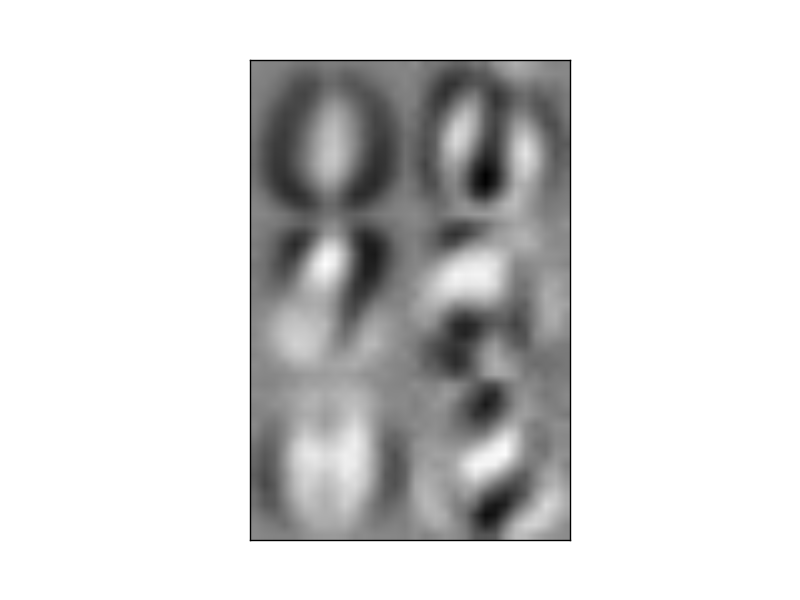
\includegraphics[width=\linewidth]{5_b_c_05.png}
  \caption{First 6 PCs}\label{fig:awesome_image3}
\endminipage
\end{figure}

\begin{figure}[H]
  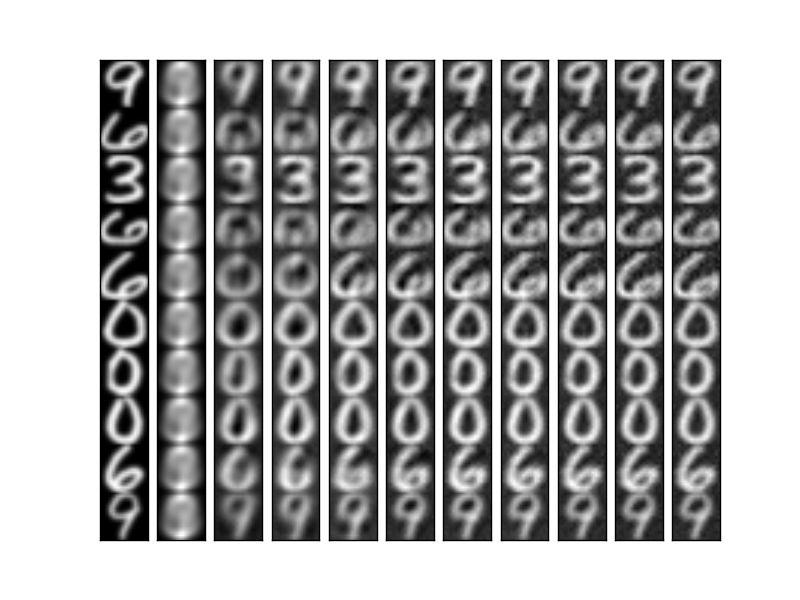
\includegraphics[width=\linewidth]{5_c_Xprime_05_45_allinone.png}
  \caption{Orginal 10 images, followed by 0, 5, 10, ... PCs}\label{fig:6}
\end{figure}


\subsection*{High noise (X + 3*noise)}
\begin{figure}[H]

\minipage{0.39\textwidth}
  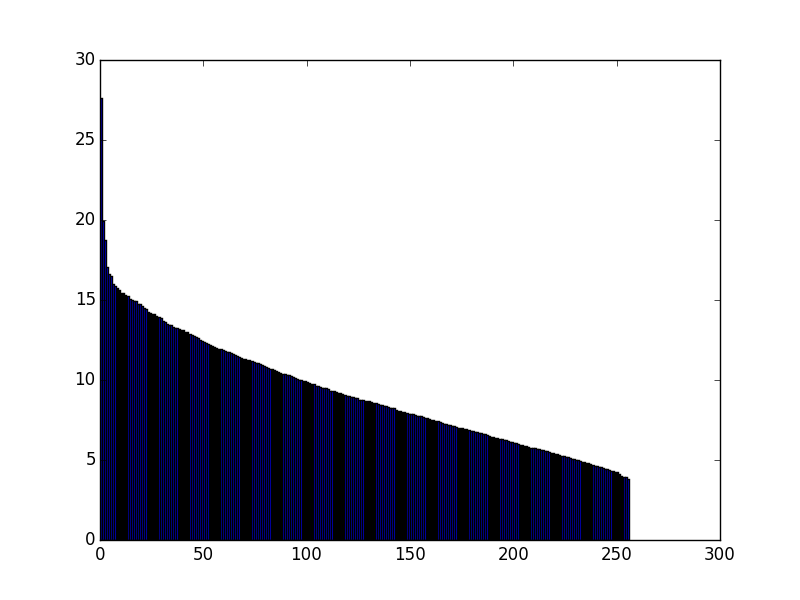
\includegraphics[width=\linewidth]{5_b_a_30.png}
  \caption{All PCs}\label{fig:awesome_image1}
\endminipage\hfill
\minipage{0.39\textwidth}
  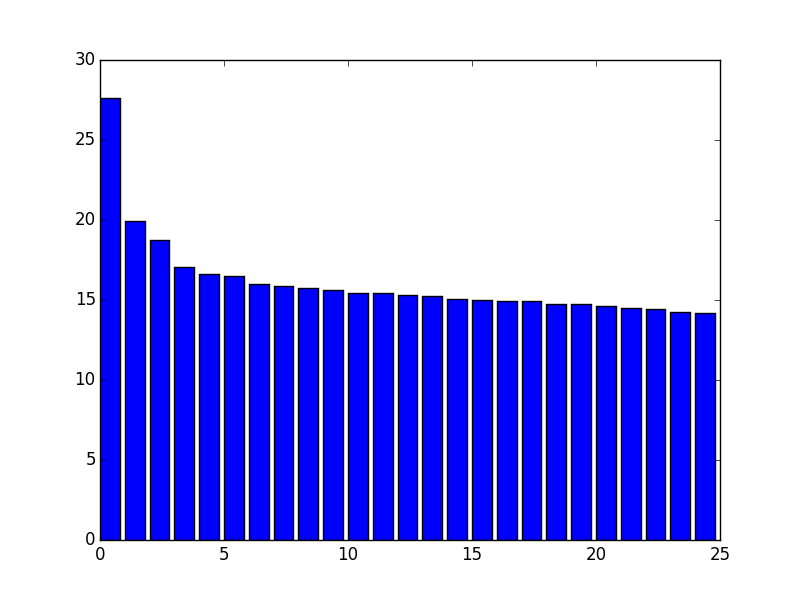
\includegraphics[width=\linewidth]{5_b_b_30.png}
  \caption{First 25 PCs}\label{fig:awesome_image2}
\endminipage\hfill
\minipage{0.20\textwidth}%
  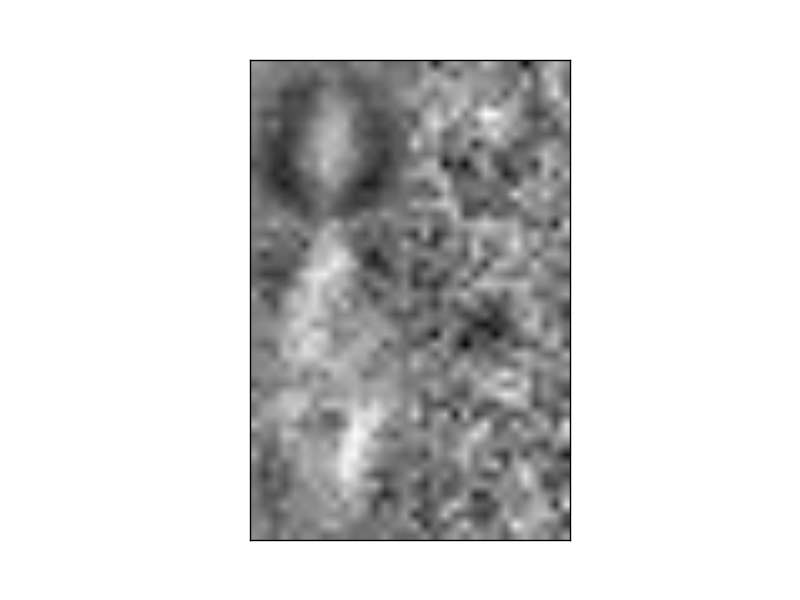
\includegraphics[width=\linewidth]{5_b_c_30.png}
  \caption{First 6 PCs}\label{fig:awesome_image3}
\endminipage
\end{figure}

\begin{figure}[H]
  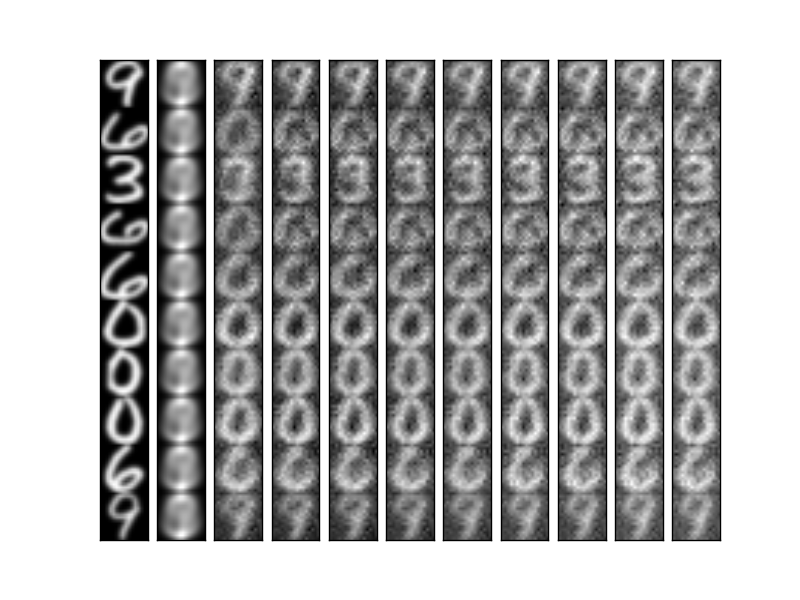
\includegraphics[width=\linewidth]{5_c_Xprime_30_45_allinone.png}
  \caption{Orginal 10 images, followed by 0, 5, 10, ... PCs}\label{fig:6}
\end{figure}

\subsection*{Outliers}
\begin{figure}[H]

\minipage{0.39\textwidth}
  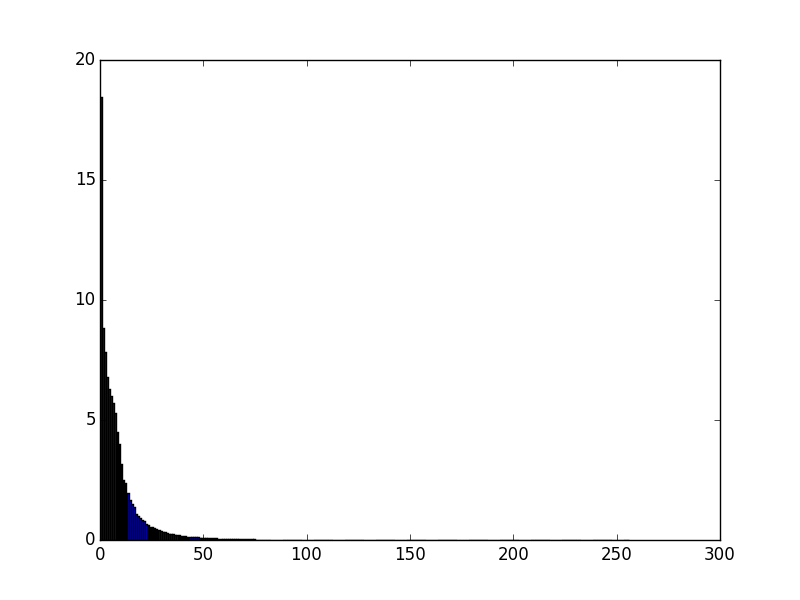
\includegraphics[width=\linewidth]{5_b_a_23479.png}
  \caption{All PCs}
\endminipage\hfill
\minipage{0.39\textwidth}
  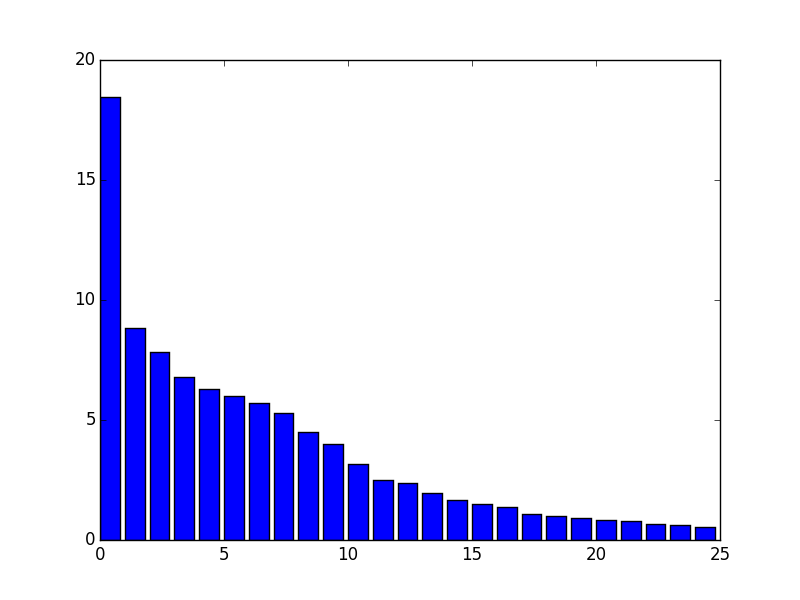
\includegraphics[width=\linewidth]{5_b_b_23479.png}
  \caption{First 25 PCs}
\endminipage\hfill
\minipage{0.20\textwidth}%
  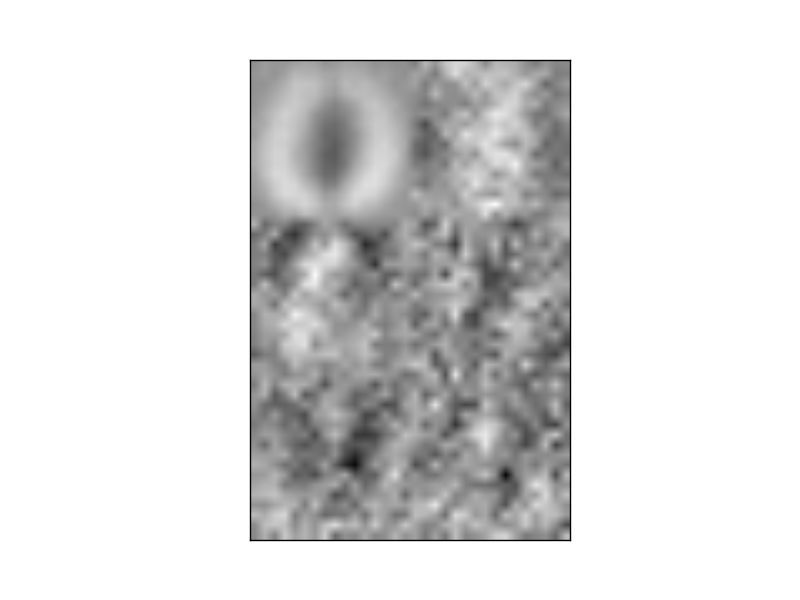
\includegraphics[width=\linewidth]{5_b_c_23479.png}
  \caption{First 6 PCs}
\endminipage
\end{figure}

\begin{figure}[H]
  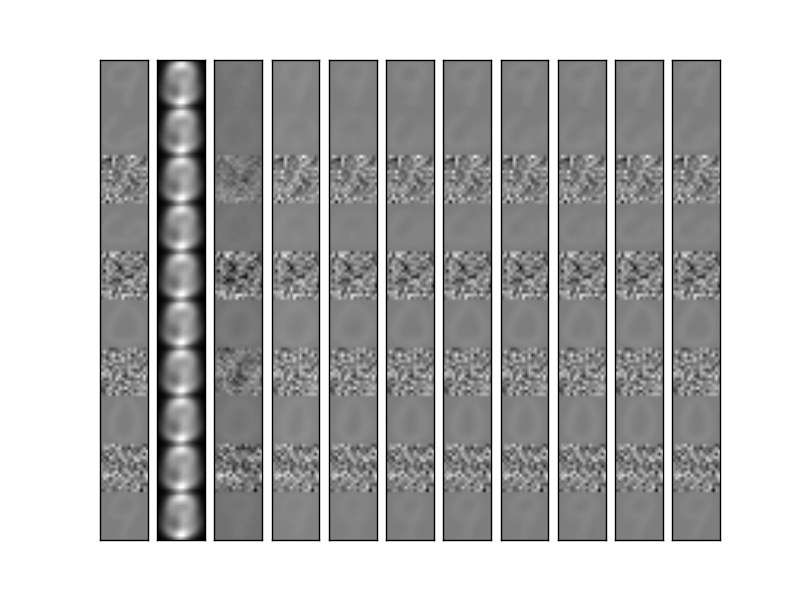
\includegraphics[width=\linewidth]{5_c_Xprime_23479_45_allinone.png}
  \caption{Orginal 10 images, followed by 0, 5, 10, ... PCs}\label{fig:6}
\end{figure}

\clearpage
\section*{Exercise 6 - Application AUC / Gamma Function}
We had big speed issues with this one.  It took 580 seconds to run each set of outliers at 100 trials each.  Almost all of the time was spent in the argsort method of our k nearest neighbors algorithm.  Our idea for speeding it up would be to first precompute the k nearest neighbors for all, then subset that, depending on which outliers were chosen.  We didn't have time to implement this though.
\begin{figure}[H]
  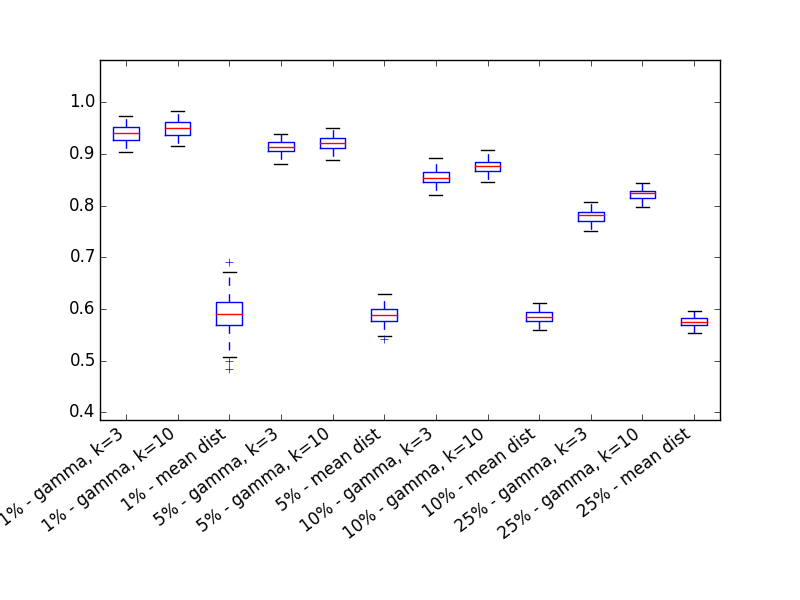
\includegraphics[width=\linewidth]{6.png}
  \caption{Outlier \% and method vs AUC}\label{fig:6}
\end{figure}

\section*{Exercise 7 - Application AUC / Gamma Function}

\begin{figure}[H]
  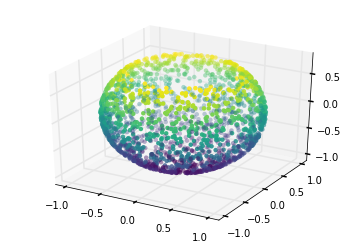
\includegraphics[width=\linewidth]{7_a_0.png}
  \caption{7.a.0}\label{fig:7_1}
\end{figure}
\begin{figure}[H]
  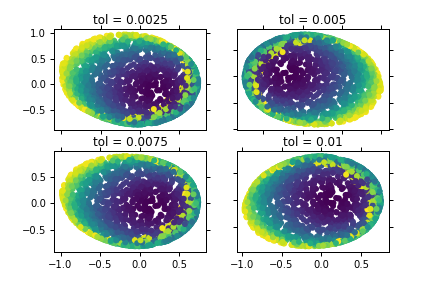
\includegraphics[width=\linewidth]{7_a_1.png}
  \caption{7.a.1}\label{fig:7_1}
\end{figure}
\begin{figure}[H]
  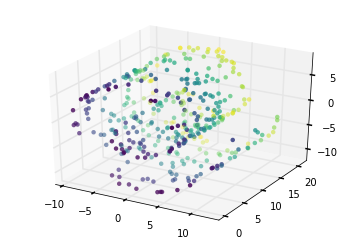
\includegraphics[width=\linewidth]{7_a_2.png}
  \caption{7.a.2}\label{fig:7_2}
\end{figure}
\begin{figure}[H]
  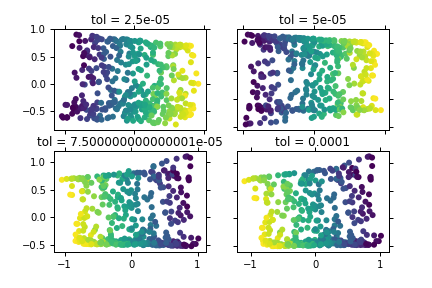
\includegraphics[width=\linewidth]{7_a_3.png}
  \caption{7.a.3}\label{fig:7_3}
\end{figure}
\begin{figure}[H]
  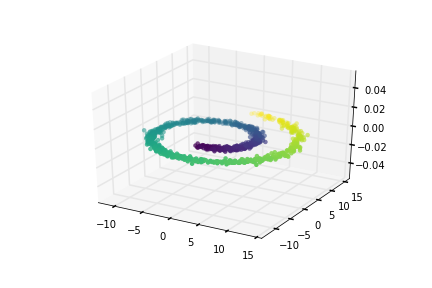
\includegraphics[width=\linewidth]{7_a_4.png}
  \caption{7.a.4}\label{fig:7_4}
\end{figure}
\begin{figure}[H]
  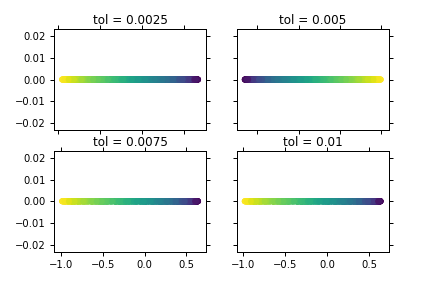
\includegraphics[width=\linewidth]{7_a_5.png}
  \caption{7.a.5}\label{fig:7_5}
\end{figure}


\end{document}